% 1.1.1
\subsubsection{Khái niệm mã hóa và giải mã}
\indent Mã hóa là quá trình chuyển đổi thông tin từ dạng có thể đọc hiểu (dữ liệu gốc) sang dạng biểu diễn không thể giải đoán hoặc nhận diện trực tiếp nếu thiếu khóa mã hóa phù hợp. Việc này giúp bảo vệ nội dung khỏi truy cập trái phép trong quá trình lưu trữ hoặc truyền đi, đảm bảo chỉ người có quyền mới đọc được dữ liệu thật từ người gửi.

\indent Ngược lại, giải mã là quá trình khôi phục lại dữ liệu ban đầu từ dạng đã mã hóa. Người nhận sẽ dùng khóa giải mã tương ứng để mở khóa dữ liệu, từ đó đọc được thông tin gốc. Đây là bước cuối cùng để đảm bảo thông tin được truyền tải an toàn, chính xác và toàn vẹn giữa các bên.

\begin{figure}[H]
  \centering
  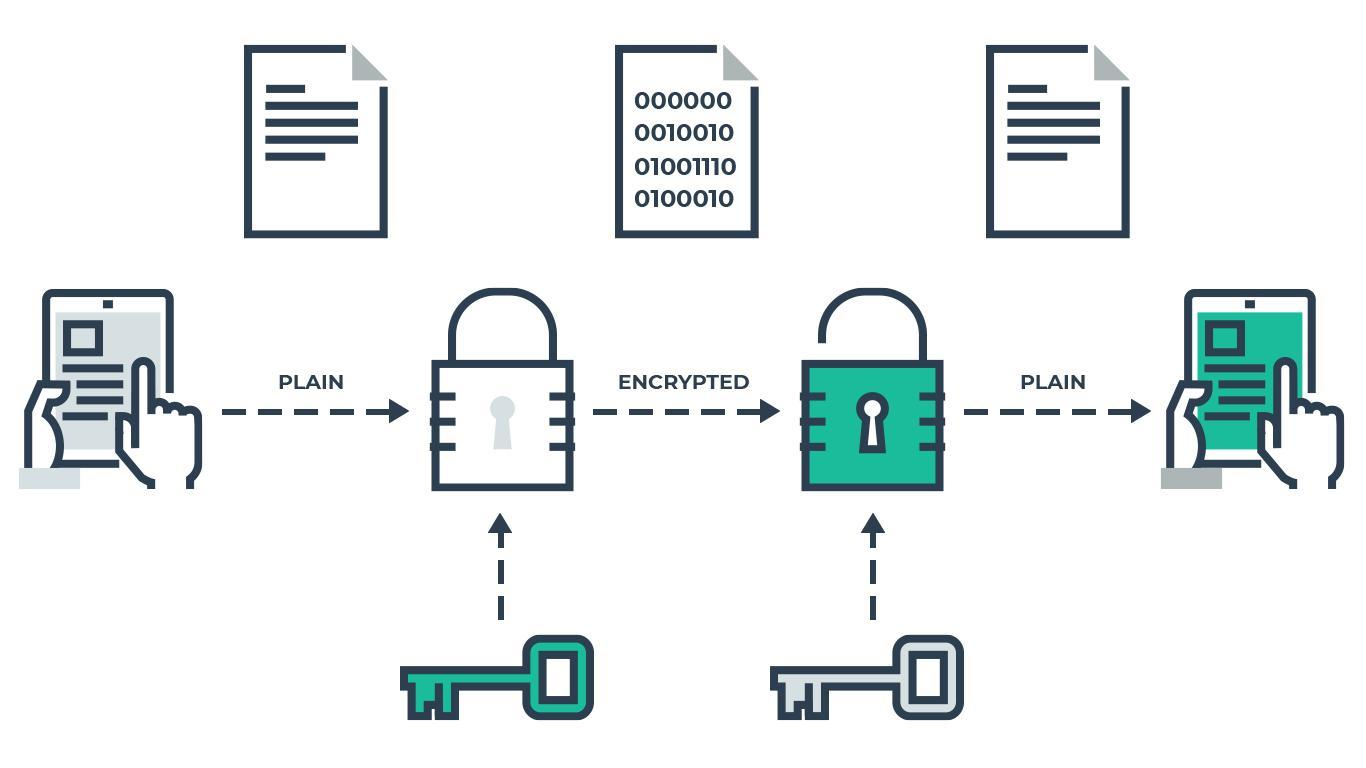
\includegraphics[width=.85\textwidth]{figures/pic1.png}
  \caption{Quy trình mã hóa và giải mã dữ liệu trong hệ thống bảo mật.}
  \label{fig:cdm1}
\end{figure}

\indent Hình ~\ref{fig:cdm1} minh họa cho thấy dữ liệu ban đầu (plain text) được khóa lại thông qua quá trình mã hóa để tạo thành dữ liệu mã hóa (cipher text). Sau đó, bên nhận sử dụng khóa giải mã tương ứng để mở khóa và khôi phục lại dữ liệu gốc. Quá trình này đảm bảo rằng chỉ người có quyền truy cập hợp lệ mới có thể đọc được thông tin, từ đó bảo vệ tính bí mật và an toàn của dữ liệu trong suốt quá trình truyền tải. Tùy thuộc vào giải thuật mã hóa đối xứng hay bất đối xứng mà khóa mã hóa và giải mã có thể giống nhau hay khác nhau.